\documentclass{beamer}

%\usetheme{Madrid}

\usepackage{float}
\usepackage{wrapfig}
\usepackage{setspace}
\usepackage{fontspec}
\usepackage{graphicx}
\usepackage{subcaption}
%\usepackage{pgfpages}\setbeameroption{show notes on second screen}

\setbeamertemplate{note page}[plain]

\setbeamertemplate{footline}{}
\setbeamertemplate{navigation symbols}{}

\setmainfont{Open Sans}
\setsansfont{Open Sans}

%\setbeamerfont{title}{size={\fontsize{18}{36}}}
\setbeamerfont{note page}{size={\fontsize{36}{72}}}

\setbeamertemplate{itemize items}[ball]

\title{Merits of Online Education}
%\title{Merits of Selective Education}
\author{Huan Li}

\begin{document}
\begin{spacing}{1.2}

\frame{\titlepage}
\note{2}

\begin{frame}
	\frametitle{Massive Open Online Course (MOOC)}
	
	%\begin{wrapfigure}{R}{0.2\textwidth}
	%	\centering
	%	
\includegraphics[width=0.25\textwidth]{mooc.eps}
	%\end{wrapfigure}
	\vspace{-9.5pt}
	\begin{figure}
		%\centering
		%
\includegraphics[width=0.6\textwidth]{mooc.eps}
		\makebox[\linewidth][c]{
		\begin{subfigure}[H]{0.48\textwidth}
			%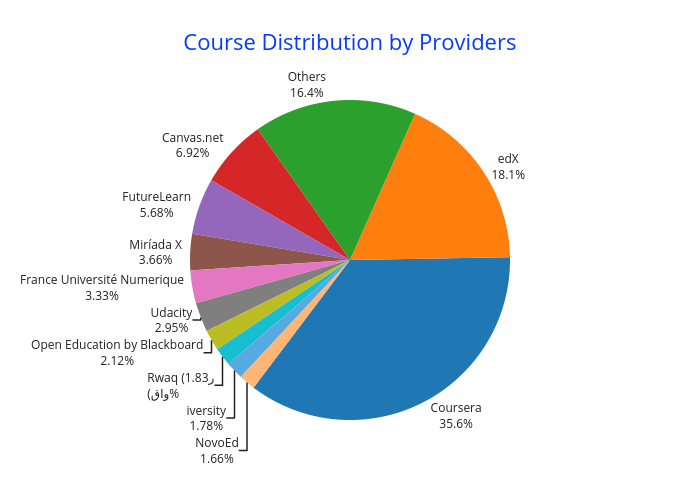
\includegraphics[width=1\textwidth]{mooc_providers2.png}
			
\includegraphics[width=1\textwidth]{mooc.png}
		\end{subfigure}
		\quad
		\begin{subfigure}[H]{0.52\textwidth}
			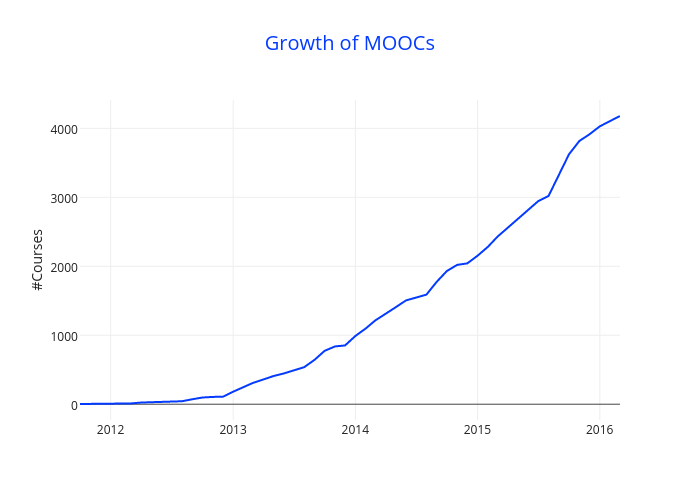
\includegraphics[width=1\textwidth]{mooc_growth2.png}
		\end{subfigure}
		}
	\end{figure}
	
	MOOC
	\begin{itemize}
		%\item Merits of MOOC
		%\begin{itemize}
			\item Encourages sharing of academic information
			\item Broadens access to education
			\item Leads to better academic performance
		%\end{itemize}
	\end{itemize}
\end{frame}

\begin{frame}
	\frametitle{Sharing of Academic Information}
\end{frame}

\begin{frame}
	\frametitle{Broad Access to Education}
\end{frame}

\begin{frame}
	\frametitle{Better Academic Performance}
\end{frame}

%\begin{frame}
%	\frametitle{Grammar schools debate}
%	\begin{itemize}
%		\item Grammar schools
%		\begin{itemize}
%			\item Schools that make admissions decisions on the basis of academic ability
%			\item In contrast to comprehensive schools
%		\end{itemize}
%		\item Merits of grammar schools
%		\begin{itemize}
%			\item 
%
%		\end{itemize}
%	\end{itemize}
%\end{frame}

\begin{frame}\end{frame}

\end{spacing}
\end{document}